\problemname{Kiki Boba}
\noindent
``\texttt{Kiki}'' och ``\texttt{boba}'' är en fascinerande ljud-symbolisk koppling, där människor spontant associerar skarpa ljud som ``\texttt{kiki}'' med taggiga former
och mjukare ljud som ``\texttt{boba}'' med rundare former. Det här avslöjar en underliggande koppling mellan ljud och visuella egenskaper, vilket ger inblick i hur
vår hjärna intuitivt skapar mening och associationer.

Fergus har länge haft ett stort intresse inom fonetik, och har utifrån denna ljud-symboliska kopplingen utvecklat en teori!
Han tror att alla ord går att dela in i 4 kategorier. Det vill säga att varje ord antingen är 
ett ord som motsvarar figuren till vänster, som ``\texttt{kiki}'', ett ord som motsvarar figuren till höger, som ``\texttt{boba}'', 
ett ord som är en blandning av båda, eller ett ord inte är något av alternativen innan.

\begin{figure}[h]
  \centering
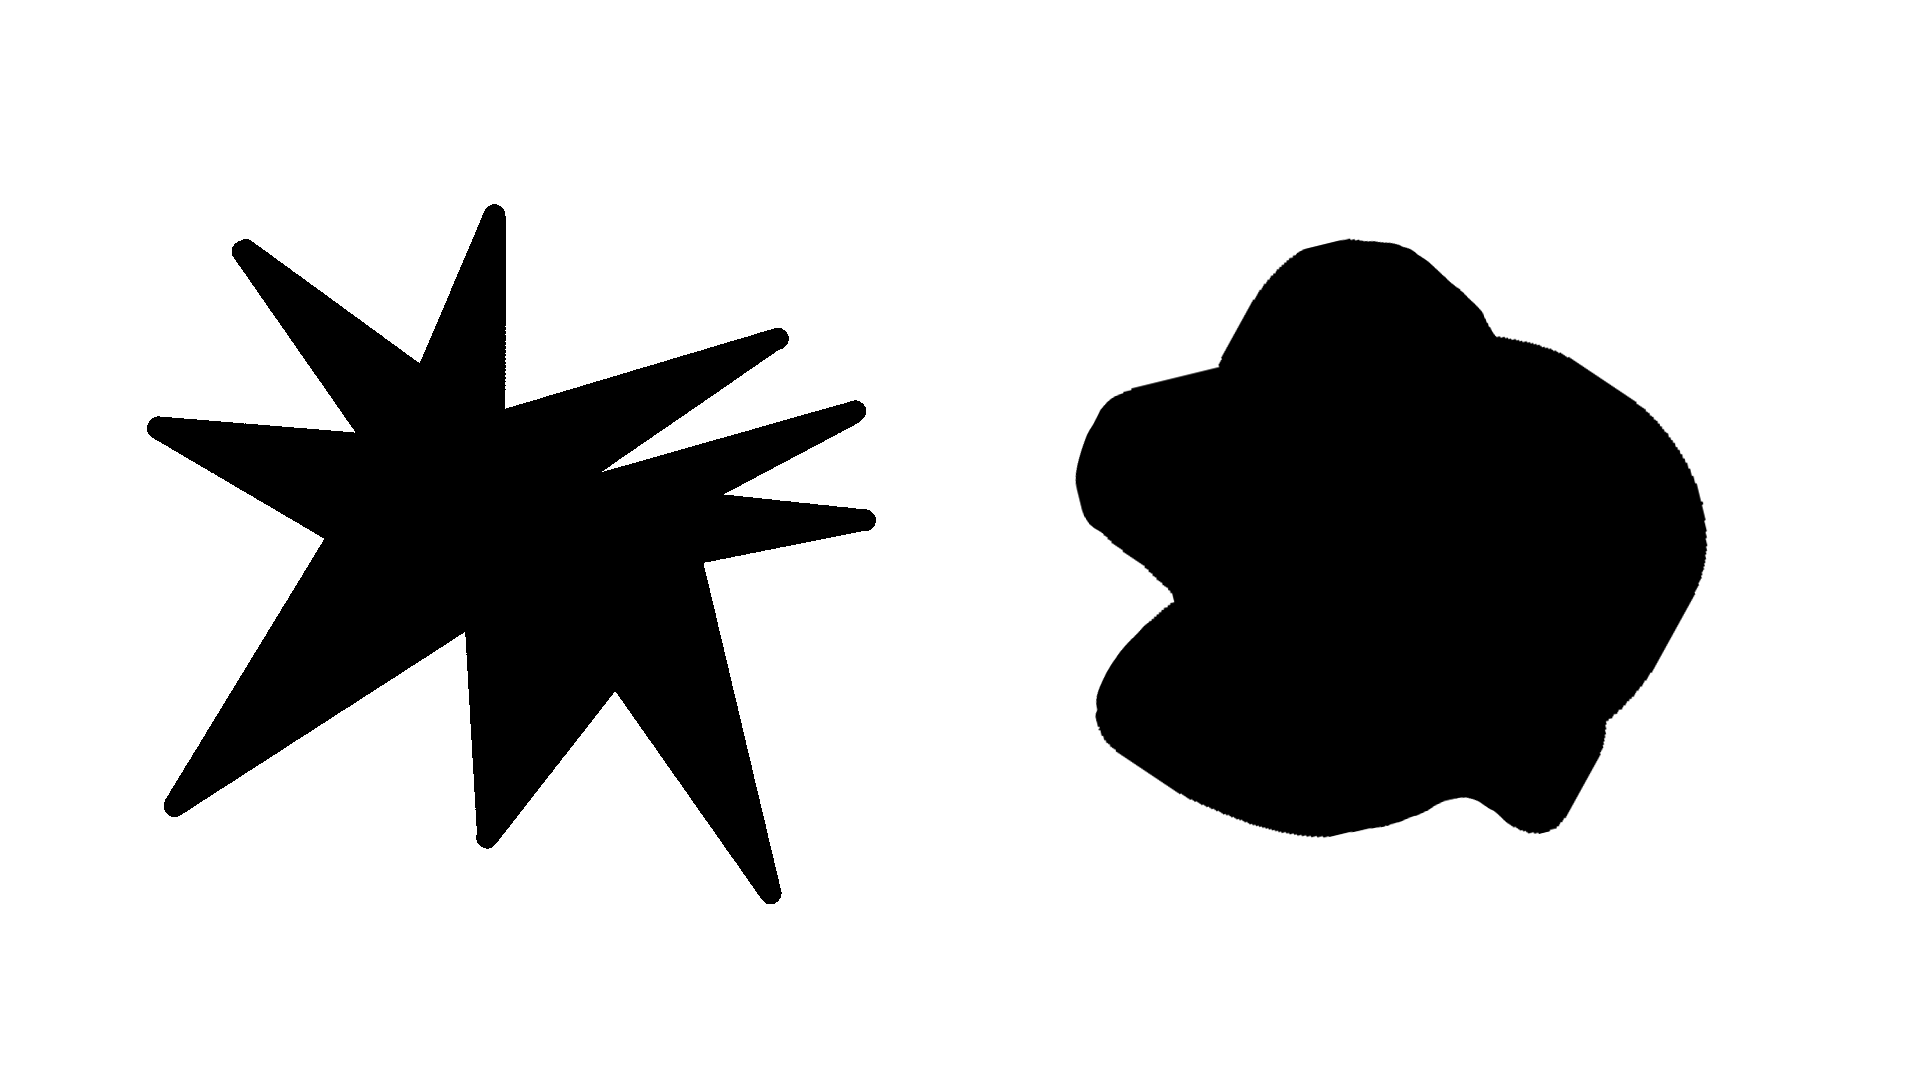
\includegraphics[width=0.6\textwidth]{kikiboba.png}
  \caption{Figur till vänster associeras vanligtvis med "kiki". Figur till höger associeras vanligtvis med "boba".}
  \label{fig:kikiboba}
\end{figure}

Fergus bestämmer att ett ord tillhör en kategori enligt följande regler:
Ifall det finns fler ``\texttt{b}'' än ``\texttt{k}'' i ordet, så är ordet ett ``\texttt{boba}''-ord.
Ifall det finns fler ``\texttt{k}'' än ``\texttt{b}'' i ordet, så är ordet ett ``\texttt{kiki}''-ord. 
Ifall ordet innehåller lika många ``\texttt{b}'' som ``\texttt{k}'', så kan kallar Fergus det ett ``\texttt{boki}''-ord.
Dessa regler håller med ett undantag: 
Ifall det varken finns ``\texttt{b}'' eller ``\texttt{k}'' i ordet, så är ordet varken nära ett ``\texttt{boba}''-ord eller ``\texttt{kiki}''-ord, och då kallas ordet ett ``\texttt{none}''-ord.

Hjälp Fergus skriva ett program som givet ett ord kan kategorisera ordet enligt Fergus regler.

\section*{Indata}
Den enda raden av indata innehåller en sträng som består av bokstäver ``\texttt{a}''-``\texttt{z}'', ordet Fergus vill kategorisera.


\section*{Utdata}
Skriv ut ett ord: antingen ``\texttt{boba}'', ``\texttt{kiki}'', ``\texttt{boki}'' eller ``\texttt{none}'', enligt Fergus regler som nämns ovan.
Det finns alltid endast en kategori som stämmer in för varje ord.

\section*{Poängsättning}
Din lösning kommer att testas på en mängd testfallsgrupper.
För att få poäng för en grupp så måste du klara alla testfall i gruppen.

\noindent
\begin{tabular}{| l | l | p{12cm} |}
  \hline
  \textbf{Grupp} & \textbf{Poäng} & \textbf{Gränser} \\ \hline
  $1$    & $20$       & Ordet är endast en bokstav långt. \\ \hline
  $2$    & $50$       & Ordet har åtminstone en av ``\texttt{k}'' eller ``\texttt{b}'', men aldrig båda samtidigt. \\ \hline
  $3$    & $30$       & Inga ytterligare begränsningar. \\ \hline
\end{tabular}

\section*{Förklaring av exempelfall 1}
Ordet innehåller 2 st ``\texttt{b}'', medan det finns inga ``\texttt{k}''. Det finns alltså fler ``\texttt{b}'' än ``\texttt{k}'', och svaret är därför ``\texttt{boba}''.

\section*{Förklaring av exempelfall 3}
Ordet innehåller 1 st ``\texttt{b}'' och 1 st ``\texttt{k}''. Det finns lika många ``\texttt{b}'' som ``\texttt{k}'', och därför är svaret ``\texttt{boki}''.
